\documentclass{../../sheet}
\renewcommand{\logopath}{../../logos/}

\title{PSE Vorkurs Tag 5}

\begin{document}
\maketitle
Heute Abend UNO!

\newpage
\aufgabe{Aufgabe 1: Maps}
Maps verbinden ein Schlüsselelement mit einem Wert. Diese können auch unterschiedliche Datentypen haben. Ein Telefonbuch könnte beispielsweise als Map dargestellt werden um Namen mit Telefeonnummern zu verbinden:
\begin{minted}[linenos=false]{java}
Map<String, Integer> telefonbuch = new HashMap<String, Integer>();
//erstes Parameter ist der Schlüssel, zweites ist der Wert
telefonbuch.put("Paul Griller", 1374927394);
\end{minted}

\begin{enumerate}
    \item
\end{enumerate}

\newpage
\aufgabe{Aufgabe 2: Datenstrukturen selber machen}
Man kann sich in Java jederzeit selbst eine eigene Datenstruktur bauen, die dann auch an die eigenheiten der Problemstellung angepasst sein kann. Ihr habt ja sicher schon gemerkt, das Arrays etwas sperrig zu nutzen sind, da deren Größe komplett statisch ist. Unsere Liste soll aus einzelnen Knotenklassen bestehen, die dann untereinander verbunden werden.
\begin{enumerate}
    \item Erstelle eine Knotenklasse namens \texttt{Node}. Jede Knotenklasse soll einen Wert \texttt{value} vom Typ \texttt{int}, sowie einen Folgeknoten \texttt{nextNode} vom Typ \texttt{Node} als Attribute haben. Erstelle einen sinnvollen Konstruktor.\\\\
    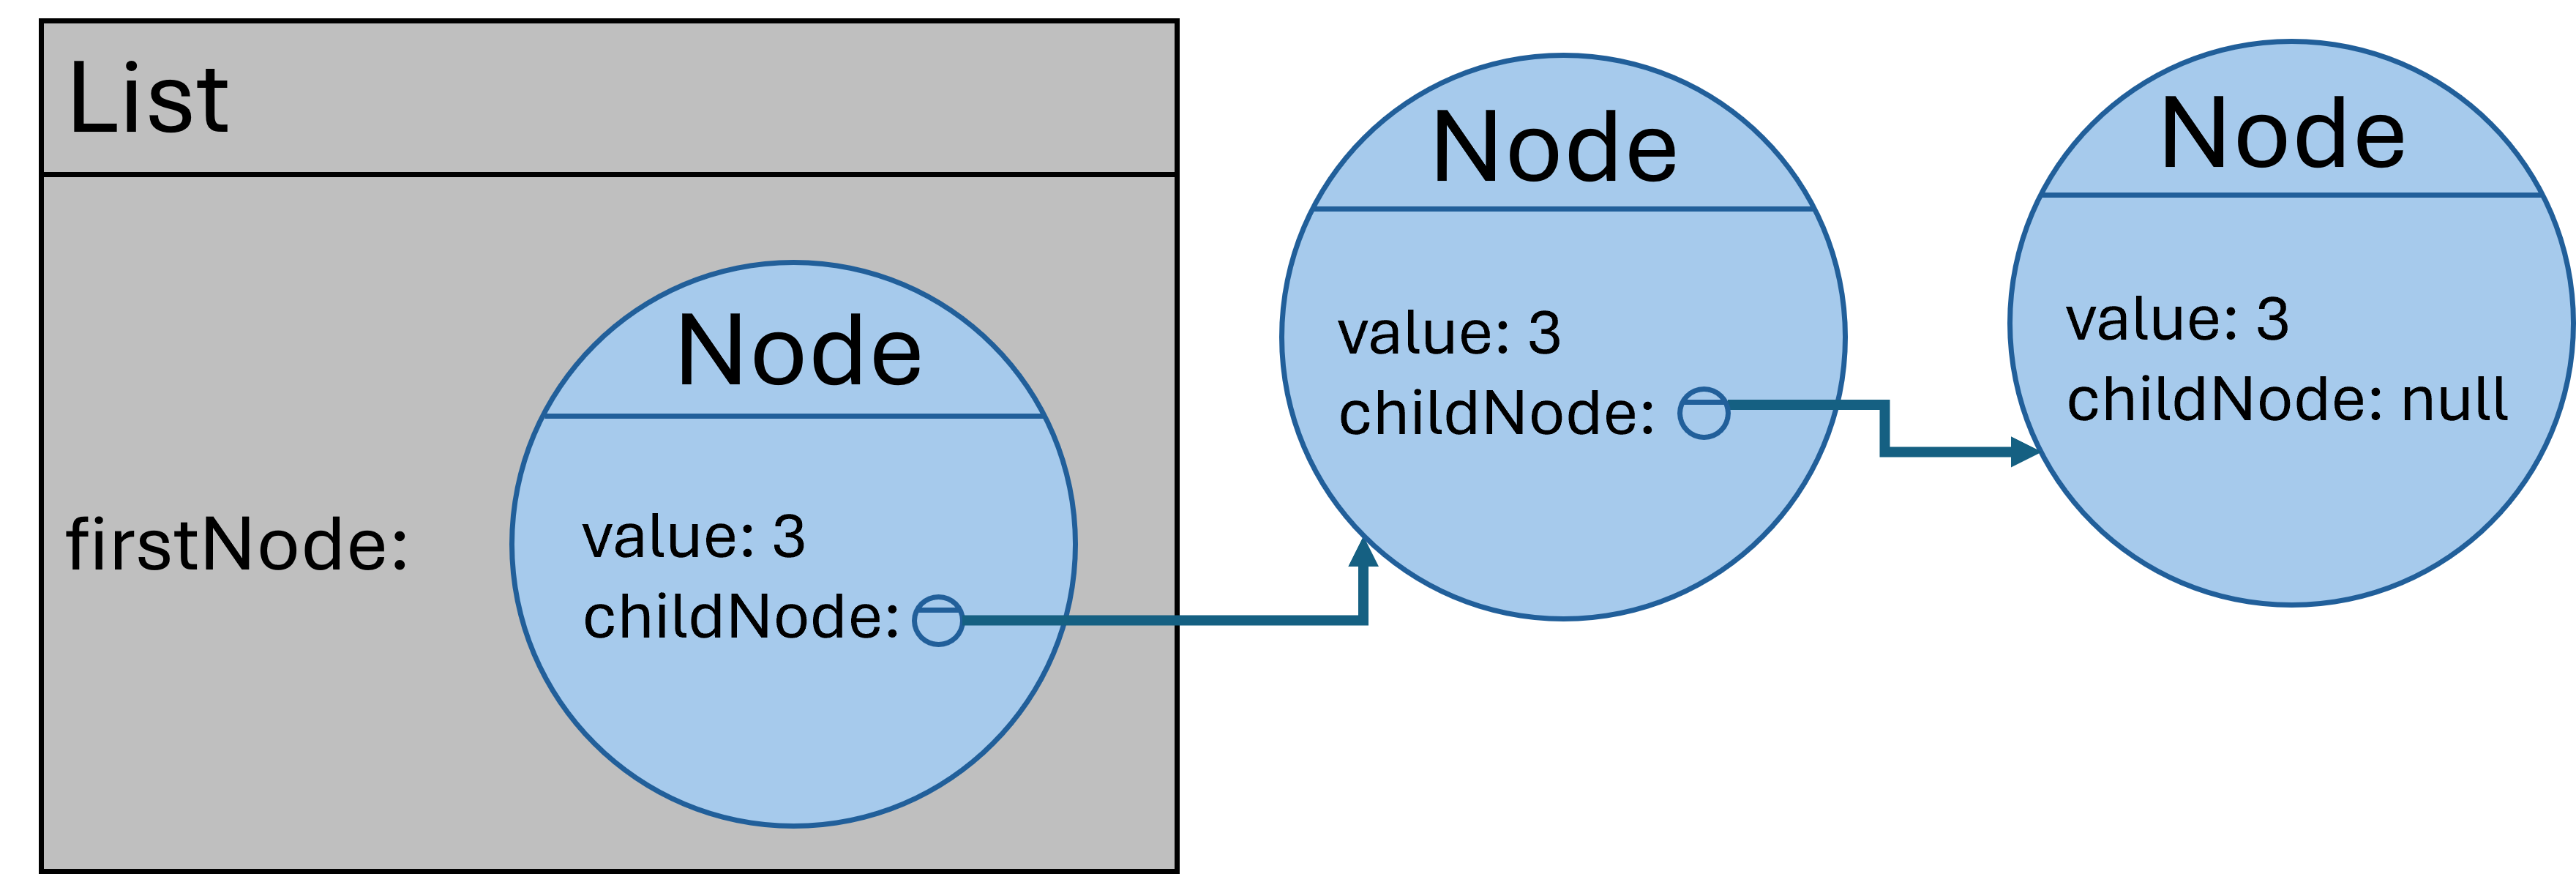
\includegraphics[width=\linewidth]{img/linkedlist.png}
    \item Erstelle jetzt die Listenklasse. Jede \texttt{List} hat einen Startknoten \texttt{startNode}. Programmiere wieder einen sinnvollen Konstruktor.
    \item Noch besteht jede dieser Listen nur aus einem einzelnen Startknoten. Füge um das zu ändern der \texttt{List} Klasse eine \texttt{add(Node newElement)} Funktion hinzu. Sie soll eine neue Node ans Ende der Liste anfügen. 
    \item Gib der \texttt{List} Klasse außerdem eine \texttt{remove(Node element)} Funktion. Achte darauf, dass dabei eventuelle Folgeelemente nicht ''Elternlos'' zurückgelassen werden. 
    \item Programmiere eine \texttt{printElements()} Funktion, die alle Elemente in der Liste anschaulich in der Konsole ausgibt.
\end{enumerate}

Du hast gerade eine einfache LinkedList programmiert. LinkedLists sind sehr wichtig als Datenstruktur mit Variabler Größe und sie existieren auch in nativem Java: \url{https://docs.oracle.com/javase/8/docs/api/java/util/LinkedList.html}

\newpage
\aufgabe{HIGHPERFORMER-Aufgabe: Bäume}
Bäume sind auch eine wichtige Datenstruktur in Java. Bei einem Baum ist jeder Knoten mit Kindknoten verbunden, welche wiederum mit weiteren Kindknoten verbunden sind. So werden die Daten in einer Baumstruktur gespeichert:
\\
\begin{center}
    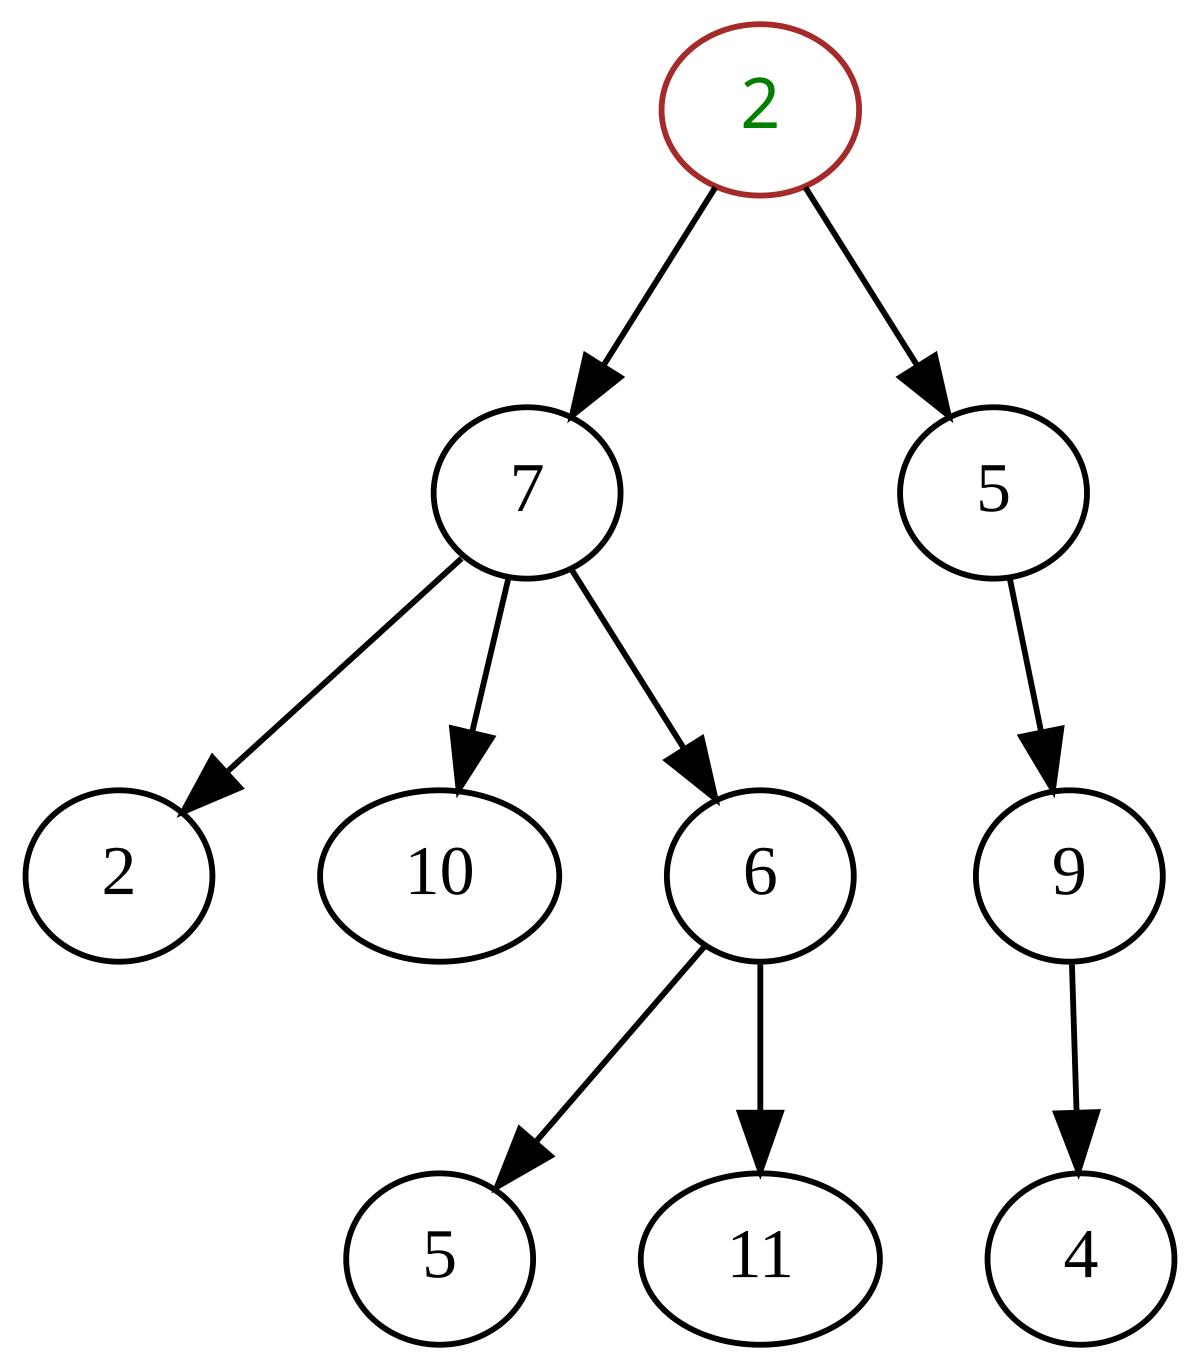
\includegraphics[width=0.5\linewidth]{img/baum.png}    
\end{center}

\begin{enumerate}
    \item Erstelle eine \texttt{Baum}-Klasse, die einen Wurzelknoten besitzt, sowie eine \texttt{Knoten}-Klasse, die einen \texttt{int}-Wert, sowie genau zwei Kindknoten (\texttt{linkesKind} und \texttt{rechtesKind}) speichert.
    \item baum printen mit max tiefe
    \item zu Array
    \item arrayzubaum
\end{enumerate}

\end{document}